\scanpage{32}
% @ 1–3
If $A$ is the algebra \tikz[baseline=(s.base)]{\node[inner sep=1pt](s){of a};\node[anchor=south east,inner sep=1pt](a) at ([xshift=2pt,yshift=7pt]s.north west){\inserted{affine}};\draw ([xshift=-8pt,yshift=-4pt]s.south west) to[out=90,in=190] ([xshift=1pt,yshift=-2pt]a.south west)--([xshift=1pt,yshift=-2pt]a.south east) to[out=0,in=-90] ([xshift=3pt,yshift=3pt]a.south east);} \unsure{monoid|monoid} \tikz[baseline=(s.base)]{\node[inner sep=1pt](s){over};\node[anchor=south east,inner sep=1pt](a) at ([xshift=2pt,yshift=7pt]s.north west){\inserted{affine $G$}};\draw ([xshift=-8pt,yshift=-4pt]s.south west) to[out=90,in=190] ([xshift=1pt,yshift=-2pt]a.south west)--([xshift=1pt,yshift=-2pt]a.south east) to[out=0,in=-90] ([xshift=3pt,yshift=3pt]a.south east);} $k$, [i.e. $A$ is equipped, in addition to the comultiplication $\unsure{\Pi|\pi}$ \tikz[baseline=(s.base)]{\node[inner sep=1pt](s){with a};\node[anchor=south east,inner sep=1pt](a) at ([xshift=2pt,yshift=7pt]s.north west){\inserted{associative and unital}};\draw ([xshift=-8pt,yshift=-4pt]s.south west) to[out=90,in=190] ([xshift=1pt,yshift=-2pt]a.south west)--([xshift=1pt,yshift=-2pt]a.south east) to[out=0,in=-90] ([xshift=3pt,yshift=3pt]a.south east);} bilinear \inserted{associative unital} multiplication \deleted{\unsure{which makes it a|which makes it a}} which is moreover \uline{commutative}, and $\Pi$ is an
% @ 4–8
algebra homomorphism] then $\forall\,k'$, the \unsure{elements|elements} of \tikz[baseline=(s.base)]{\node[inner sep=1pt](s){$\mathrm{Hom}_{k\text{-mod.}}(A,k')$};\node[anchor=south east,inner sep=1pt](a) at ([xshift=2pt,yshift=7pt]s.north west){\inserted{$V(A)(k')=$}};\draw ([xshift=-8pt,yshift=-4pt]s.south west) to[out=90,in=190] ([xshift=1pt,yshift=-2pt]a.south west)--([xshift=1pt,yshift=-2pt]a.south east) to[out=0,in=-90] ([xshift=3pt,yshift=3pt]a.south east);} \tikz[baseline=(s.base)]{\node[inner sep=1pt](s){are};\node[anchor=south east,inner sep=1pt](a) at ([xshift=2pt,yshift=7pt]s.north west){\inserted{i.e. the $k$-linear homomorphisms $A\to k'$}};\draw ([xshift=-8pt,yshift=-4pt]s.south west) to[out=90,in=190] ([xshift=1pt,yshift=-2pt]a.south west)--([xshift=1pt,yshift=-2pt]a.south east) to[out=0,in=-90] ([xshift=3pt,yshift=3pt]a.south east);} \unsure{called|called} the ``\uline{distributions} of $G$ with \deleted{\unsure{values}} coefficients in $k'$'', denoted $\mathrm{Dist}(G)(k')$\tikz[baseline=(s.base)]{\node[inner sep=1pt](s){.};\node[anchor=south east,inner sep=1pt](a) at ([xshift=2pt,yshift=7pt]s.north west){\inserted{[algebra of distributions]}};\draw ([xshift=-8pt,yshift=-4pt]s.south west) to[out=90,in=190] ([xshift=1pt,yshift=-2pt]a.south west)--([xshift=1pt,yshift=-2pt]a.south east) to[out=0,in=-90] ([xshift=3pt,yshift=3pt]a.south east);} Thus \deleted{\unsure{we have}} they form a $k'$-algebra [``the algebra of the \deleted{group} \inserted{monoid} \deleted{\unsure{G}} $G$ with coefficients in $k'$''] and we shall have an \unsure{inclusion|the inclusion} of monoids
% @ 9
\[
 G\deleted{(k')}\hookrightarrow\mathrm{Dist}(G)(k')^{\unsure{\times|x}}
\]
% @ 10–11
and if $G$ is a group
\[
 G(k')\hookrightarrow\mathrm{Dist}(G)(k')^{*}
\]
\margin{\tikz[baseline=-.2ex,x=1em,y=1em]{\draw (.36,.77)--(.12,.77)--(.12,-.08)--(.34,-.08); \draw (.12,.68) to[out=-125,in=180] (.09,-.01) to[out=-10,in=0] (.30,-.11);}\unsure{practically|practically} never an isomorphism]}

% @ 11 left margin
% margin note written sideways
\margin{\diagram{\rotatebox{90}{\begin{tikzcd}[ampersand replacement=\&,column sep=small,row sep=small,font=\scriptsize]
 \mathrm{Dist}(X) \arrow[r,"{\Pi}"] \& \mathrm{Dist}(X)\times\mathrm{Dist}(X) \& \Pi(x)={} \\
 \deleted{e} \arrow[r,phantom,"{\deleted{\to}}"] \& \deleted{\mathrm{Dist}(X)} \& \\
 e \arrow[uu] \& \&
\end{tikzcd}}}}

% @ 12–13
\figure{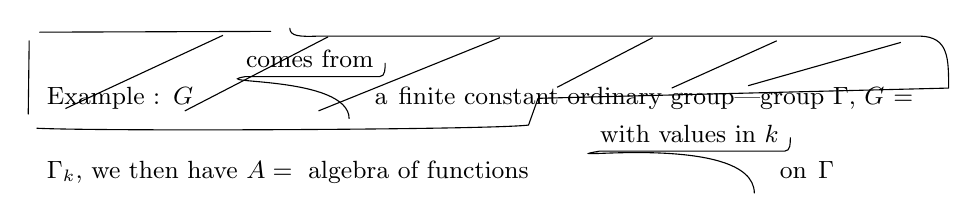
\begin{tikzpicture}[x=\linewidth,y=1cm]
\node[anchor=north west,inner sep=0pt,text width=.92\linewidth,font=\small] at (.025,.02)
 {\deleted{Example : $G$ \tikz[baseline=(s.base)]{\node[inner sep=1pt](s){a};\node[anchor=south east,inner sep=1pt](a) at ([xshift=2pt,yshift=7pt]s.north west){\inserted{comes from}};\draw ([xshift=-8pt,yshift=-4pt]s.south west) to[out=90,in=190] ([xshift=1pt,yshift=-2pt]a.south west)--([xshift=1pt,yshift=-2pt]a.south east) to[out=0,in=-90] ([xshift=3pt,yshift=3pt]a.south east);} finite \deleted{constant} \inserted{ordinary} \unsure{group|group} $\Gamma$, $G=\Gamma_k$, we then have $A={}$ algebra of functions \tikz[baseline=(s.base)]{\node[inner sep=1pt](s){on};\node[anchor=south east,inner sep=1pt](a) at ([xshift=2pt,yshift=7pt]s.north west){\inserted{with values in $k$}};\draw ([xshift=-8pt,yshift=-4pt]s.south west) to[out=90,in=190] ([xshift=1pt,yshift=-2pt]a.south west)--([xshift=1pt,yshift=-2pt]a.south east) to[out=0,in=-90] ([xshift=3pt,yshift=3pt]a.south east);} $\Gamma$}};
\draw[line cap=round,line join=round] (.018,.21) -- (.26,.22)
 (.28,.26) .. controls (.28,.16) and (.29,.15) .. (.31,.16)
 -- (.94,.16) .. controls (.97,.15) and (.97,-.12) .. (.97,-.50)
 -- (.54,-.63) -- (.53,-.97) .. controls (.49,-1.03) and (.08,-1.05) .. (.015,-1.01)
 (.006,-.83) -- (.007,.10);
\draw (.045,-.76)--(.21,.17) (.17,-.79)--(.32,.15)
 (.31,-.79)--(.50,.14) (.56,-.49)--(.66,.14)
 (.68,-.50)--(.79,.10) (.76,-.47)--(.92,.08);
\end{tikzpicture}}

% @ 14–17
\[
 gg^{-1}=1
\]
\diagram{\begin{tikzcd}[ampersand replacement=\&,column sep=large]
 G \arrow[dr,"{\dot p}"] \arrow[r,dash,"{\mathrm{id}_G\times\sigma}",to path={-- (\tikztotarget) \tikztonodes (\tikztostart) ++(1.8pt,-.8pt)--++(1.6pt,2.5pt) (\tikztotarget) ++(0pt,-1.2pt)--++(0pt,2.4pt)}] \& G\times G \arrow[r,"{\Pi}",dash,to path={-- (\tikztotarget) \tikztonodes (\tikztotarget) ++(0pt,-1.3pt)--++(0pt,2.5pt)}] \& G \\
 \& e \arrow[ur,"{\varepsilon}"] \&
\end{tikzcd}}
% @ 15 opposite first diagram
\[
 \deleted{A\to A\otimes A}
\]

% @ 18–21
\diagram{\begin{tikzcd}[ampersand replacement=\&,column sep=large]
 x\sigma y \& (x,y) \arrow[l,maps to] \& \\
 A \& A\otimes A \arrow[l,dash,to path={-- (\tikztotarget) \tikztonodes (\tikztotarget)--++(3pt,3pt) (\tikztotarget)--++(3pt,-2.5pt) (\tikztotarget) ++(2.3pt,0pt) to[out=110,in=-120] ++(1pt,2pt) (\tikztotarget) ++(2.3pt,0pt)--++(1pt,-1.1pt)}] \& A \arrow[l,"{\Pi}"] \arrow[dl,"{\varepsilon}"] \\
 \& k \arrow[ul,"p"] \&
\end{tikzcd}}
% @ 18–21 left margin
% margin note written sideways
\margin{\diagram{\rotatebox{90}{\begin{tikzcd}[ampersand replacement=\&,column sep=small,row sep=small,font=\scriptsize]
 \deleted{X\times Y}\;A \arrow[dr,"{\varepsilon}"'] \& A\otimes A \arrow[l] \arrow[d,shift left] \arrow[d,shift right,to path={-- (\tikztotarget) \tikztonodes},execute at end to={\draw ([yshift=-5pt]\tikztostart) to[out=-135,in=160] ([yshift=-11pt]\tikztostart); \fill ([xshift=-2pt,yshift=-4pt]\tikztotarget) circle (.45pt);}] \& x\otimes y \\
 \& k \& \unsure{\varepsilon(x)\varepsilon(y)|\varepsilon x)\varepsilon y)}
\end{tikzcd}}}}
% archive sheet number: 31
